%!TEX root = ../report.tex

\todo{Purpose of the chapter
 Structure of the chapter
 Central themes of the chapter}

\section{Flat surface} {
\label{sec:flat_surface}
	
}

\section{Round surface} {
\label{sec:round_surface}
	
}

\section{Grid} {
\label{sec:grid}
	
}

\section{Navigation} {
\label{sec:navigation}

	The navigation techniques that the user can interact with are: pan, rotate and zoom. This functionality was implemented in a single module and utilised mouse events to detect when the user was scrolling or pressing the left or right mouse button. It is important to note that Three.js uses a right-handed coordinate system, as shown in Figure~\ref{fig:threejs_coordinate_system}.

	%!TEX root = ../../report.tex

\begin{figure}[H]
	\centering
	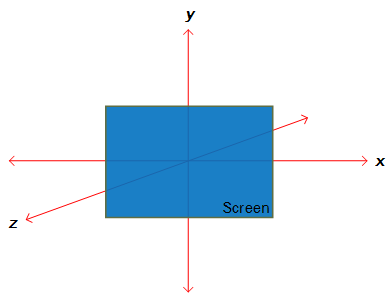
\includegraphics{images/implementation/threejs_coordinate_system}
	\caption[Three.js coordinate system]{Three.js coordinate system\protect\footnotemark.}
	\label{fig:threejs_coordinate_system}
\end{figure}

\footnotetext{\bibentry{microsoft2015threejs}}


	\subsection{Pan} {
	\label{sec:pan}

		This interaction is initiated when a \texttt{mousedown} event is fired on the canvas, followed by a \texttt{mousemove} event bound to the \texttt{window}. This simulates drag when pressing the left mouse button.

		As the user moves their pointer, the camera is translated in the x and y direction. This calculation relies on converting screen coordinates to world coordinates and normalising the value so it is a ratio of the viewport height, instead of both the width and height.

		Once the translation to the camera has been applied, the \texttt{origin} vector needs to be updated, which is used during rotation. An updated origin ensures there is no sudden movement when rotating, after panning the screen.

		Finally, when the user releases the left mouse button, a \texttt{mouseup} event is triggered which removes the event binding for \texttt{mousemove} on the \texttt{window}. 

	}

	\subsection{Rotate} {
	\label{sec:rotate}

		Rotation uses the same event chain as panning, except instead of listening to the left mouse click, it listens to the right.

		To rotate the camera, the cartesian coordinates need to be calculated from spherical coordinates, using the following formula in a right-handed mathetmatics system:

		%!TEX root = ../../report.tex

\begin{gather*}
	x = r\sin\phi\sin\theta \\
	y = r\cos\phi \\
	z = r\sin\phi\cos\theta
	\intertext{Where:}
	\begin{tabularx}{\textwidth}{@{}>{$}r<{$}@{\ :\ }X@{}}
		r & is the radial distance of the camera from the origin. \\
		\phi & is the polar angle, calculated by adding the delta phi angle with the angle from the y-axis. \\
		\theta & is the azimuthal angle, calculated by adding the delta theta angle with the angle from the z-axis around the y-axis. \\
	\end{tabularx}
\end{gather*}
	
	}

	\subsection{Zoom} {
	\label{sec:zoom}

		This navigation technique begins when a \texttt{wheel} event is triggered from the browser. A ratio of the delta value is taken and the camera is then translated by this amount.
	
	}

}

\section{Filtering} {
\label{sec:filtering_implementation}

	Filtering was implemented using an event-driven approach 

	\todo{say how filtering was done, issues with extending it when I get around to implementing...should be a simple show/hide technique based on value}

	%!TEX root = ../../report.tex

\begin{figure}[H]
	\centering
	\figureborder{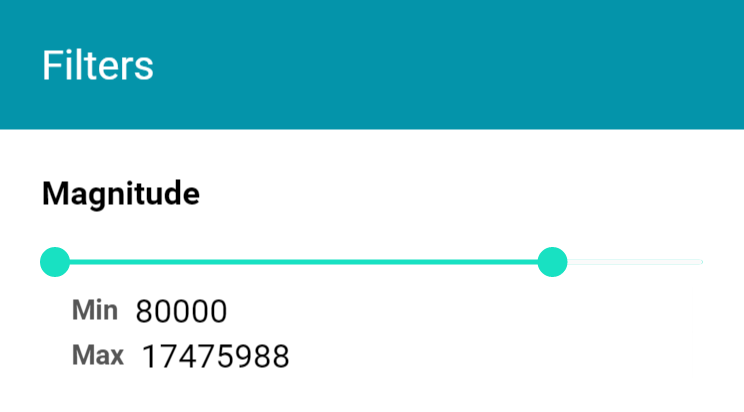
\includegraphics{images/implementation/filters}}
	\caption[Filtering]{Example of filtering.}
	\label{fig:filtering}
\end{figure}


}

\section{Configuration} {
\label{sec:configuration_implementation}

	Real-time configurations are best achieved by using shaders. Shaders are computer programs that perform shading on a graphics processing unit (GPU), making them highly efficient and well suited to parallel processing~\footnote{\bibentry{gerdelan2014shaders}}. Three.js provides abstracted materials that use shaders in the background, but this method does not easily facilitate highly customisable configurations or filter effects. Therefore, custom shaders were designed and implemented for the system to maximise efficiency and flexibility. An example of the available effects that were implemented in the system is shown in Figure~\ref{fig:shaders}.

	%!TEX root = ../../report.tex

\begin{figure}[H]
	\captionsetup[subfigure]{aboveskip=-0.8em,belowskip=0.5em}
	\newcommand{\figurewidth}{0.5\textwidth}
	\begin{subfigure}[b]{\figurewidth}
        \figureborder{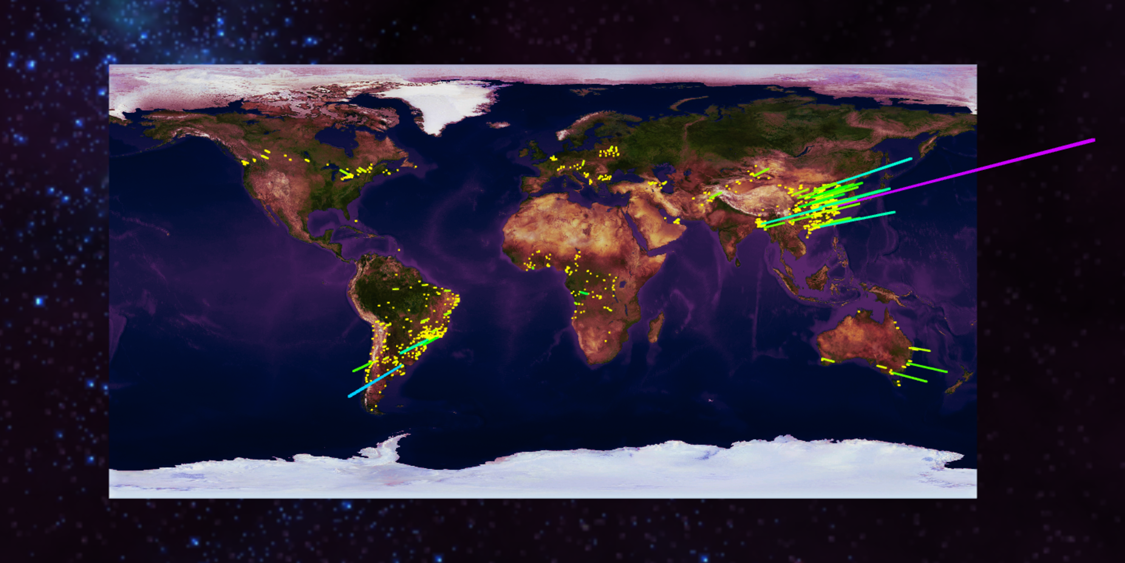
\includegraphics[width=\textwidth]{images/implementation/shaders/red}}
		\caption{Red midtone filter effect.}
		\label{fig:red_midtone}
	\end{subfigure}
	\begin{subfigure}[b]{\figurewidth}
		\figureborder{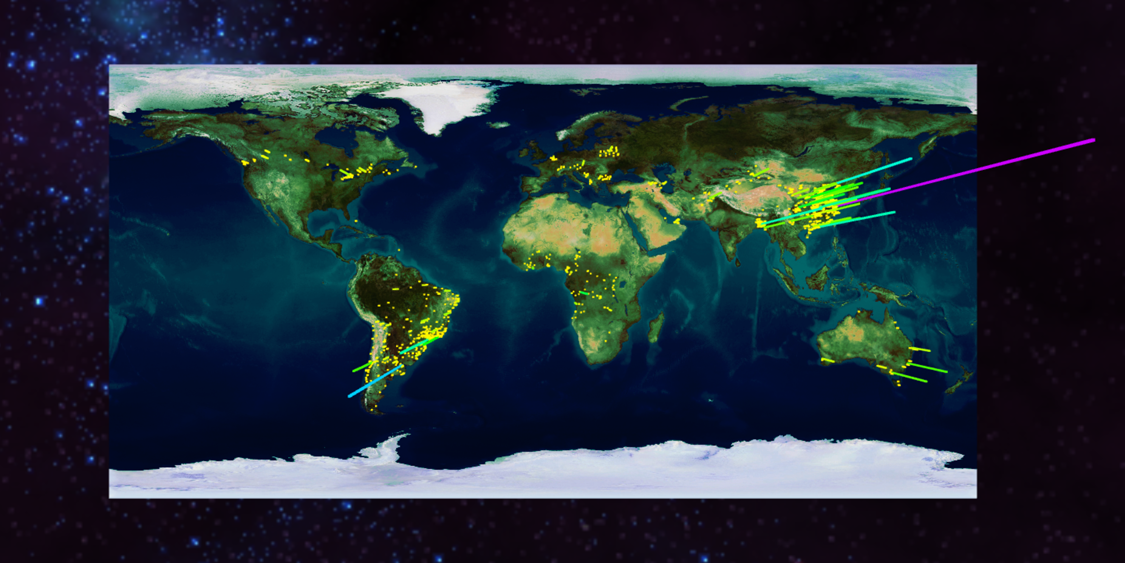
\includegraphics[width=\textwidth]{images/implementation/shaders/green}}
		\caption{Green midtone filter effect.}
		\label{fig:green_midtone}
	\end{subfigure}
	\begin{subfigure}[b]{\figurewidth}
		\figureborder{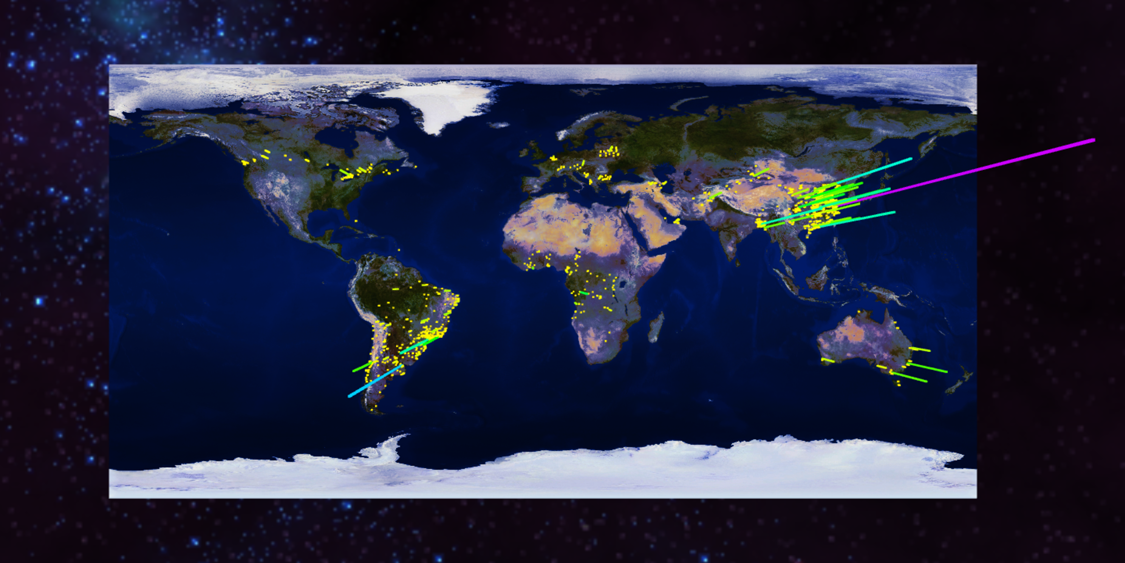
\includegraphics[width=\textwidth]{images/implementation/shaders/blue}}
		\caption{Blue midtone filter effect.}
		\label{fig:blue_midtone}
	\end{subfigure}
	\begin{subfigure}[b]{\figurewidth}
		\figureborder{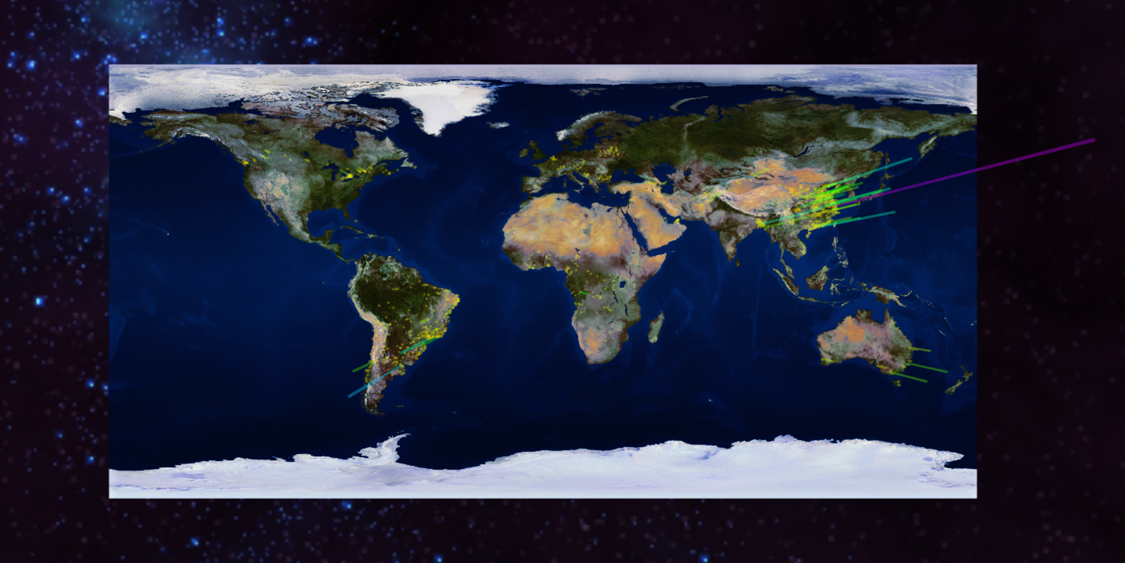
\includegraphics[width=\textwidth]{images/implementation/shaders/opacity}}
		\caption{Opacity filter effect.}
		\label{fig:opacity_filter}
	\end{subfigure}
	\begin{subfigure}[b]{\figurewidth}
		\figureborder{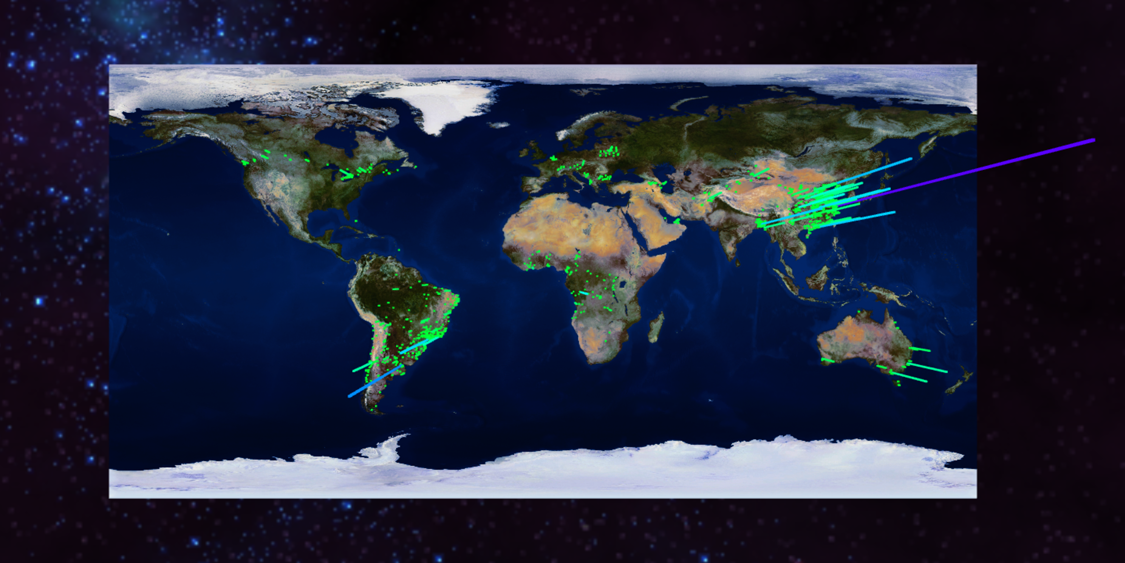
\includegraphics[width=\textwidth]{images/implementation/shaders/basic}}
		\caption{Alternate HSV colour range.}
		\label{fig:hsv_colour}
	\end{subfigure}
	\begin{subfigure}[b]{\figurewidth}
		\figureborder{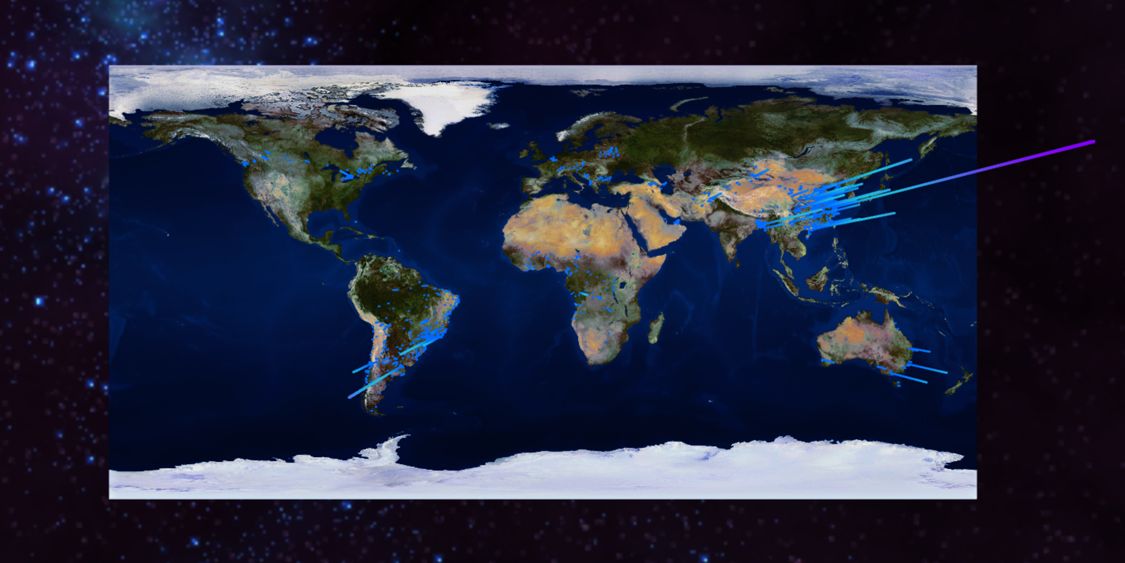
\includegraphics[width=\textwidth]{images/implementation/shaders/gradient}}
		\caption{Alternate gradient colour scheme.}
		\label{fig:gradient_colour}
	\end{subfigure}
	\caption[Shaders]{Available shader filter effects.}
	\label{fig:shaders}
\end{figure}


	These configurations can be adjusted in real-time with \href{http://workshop.chromeexperiments.com/}{dat.GUI}, a lightweight GUI for changing JavaScript variables in real-time. This tool is easy to use, setup and can modify shader uniforms automatically or by implementing \texttt{onChange} event handlers. dat.GUI can constrain input data and provides widgets for modifying values, colours and combo boxes. While this tool is great for modifying data on the fly, it has an outdated interface that does not always adapt well to particular colour schemes and designs. For this reason, the dat.GUI styles were modified to seamlessly integrate with the current system and the Material Design standards. The differences in design can be compared in Figure~\ref{fig:dat_gui} below.

	%!TEX root = ../../report.tex

\begin{figure}[H]
	\newcommand{\figurewidth}{0.4\textwidth}
	\newcommand{\figureheight}{7cm}
	\centering
	\begin{subfigure}[b]{\figurewidth}
        \figureborder{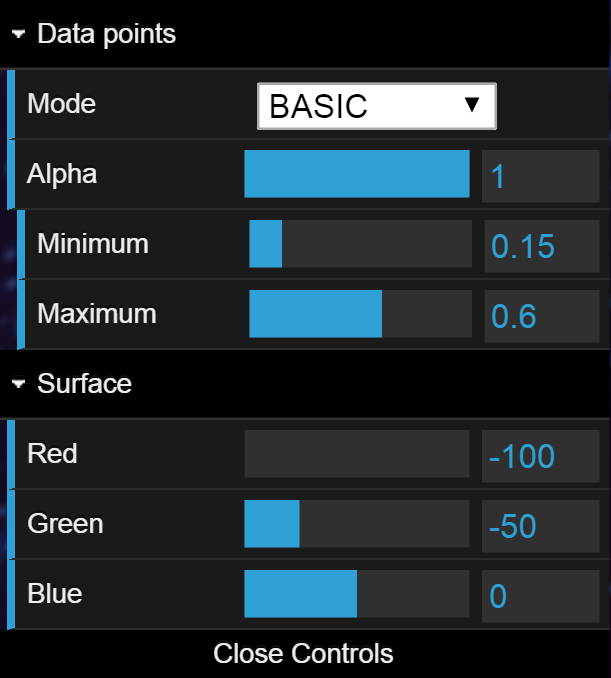
\includegraphics[width=\textwidth,height=\figureheight]{images/implementation/dat_gui/before}}
		\caption{Original dat.GUI interface.}
		\label{fig:dat_gui_before}
	\end{subfigure}
	\begin{subfigure}[b]{\figurewidth}
		\figureborder{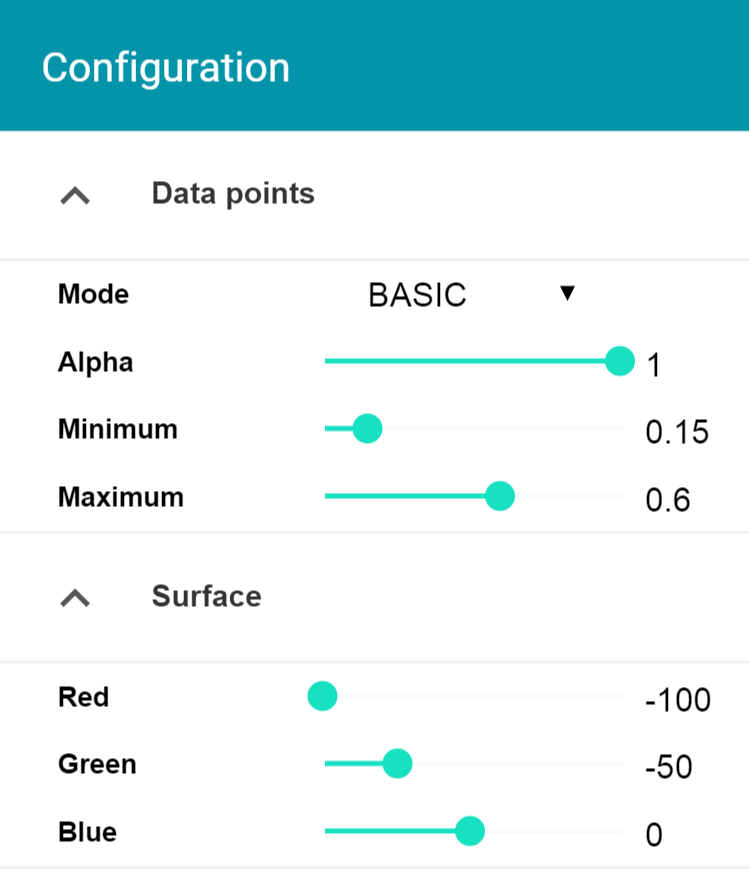
\includegraphics[width=\textwidth,height=\figureheight]{images/implementation/dat_gui/after}}
		\caption{dat.GUI interface after custom styling.}
		\label{fig:dat_gui_after}
	\end{subfigure}
	\caption[dat.GUI interface]{dat.GUI interface.}
	\label{fig:dat_gui}
\end{figure}


	The design for these configurations were continually refined during implementation. Initially, the dat.GUI sliders were to remain unchanged. However, these sliders proved to be inconsistent in regards to the colour scheme and filter design. Furthermore, the bold folder colours were eventually removed to reflect drawer layouts that conform to using light navigation colours, hover effects, and left floated icons.

}

\section{Data display} {
\label{sec:data_display}

	\todo{write about how the data displays were implemented - bunch of cubegeoms that get updated}

	% The development of these visualisations will involve using the established \href{http://threejs.org/docs/#Reference/Extras.Geometries/BoxGeometry}{BoxGeometry} and NURBS surface that are available in Three.js. The \href{http://threejs.org/examples/webgl_geometry_nurbs.html}{NURBS example}, as displayed in Appendix~\ref{app:nurbs}, proves that it is possible to render a smooth 3D surface. This can be applied to represent a heat map and if there lie difficulties in implementing this, then a simpler representation can be modelled.

}

\section{Information display} {
\label{sec:information_display}

	\todo{say how this was implemented - raycaster in requestanimframe, toggles one element to hide/show so nothing new in dom is added (more performant)}

	%!TEX root = ../../report.tex

\begin{figure}[H]
	\centering
	\newcommand{\figurewidth}{0.4\textwidth}
	\centering
	\begin{subfigure}[b]{\figurewidth}
        \figureborder{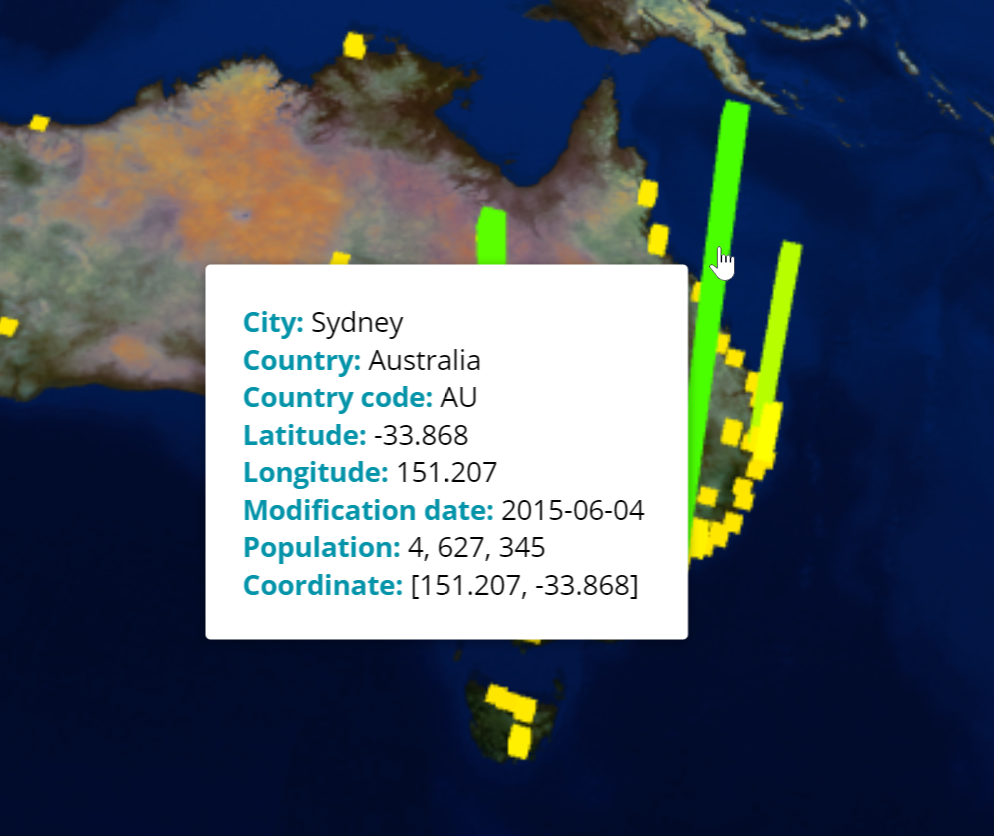
\includegraphics[width=\textwidth]{images/implementation/information_display/population}}
		\caption{Information display for population data.}
		\label{fig:information_display_population}
	\end{subfigure}
	\begin{subfigure}[b]{\figurewidth}
		\figureborder{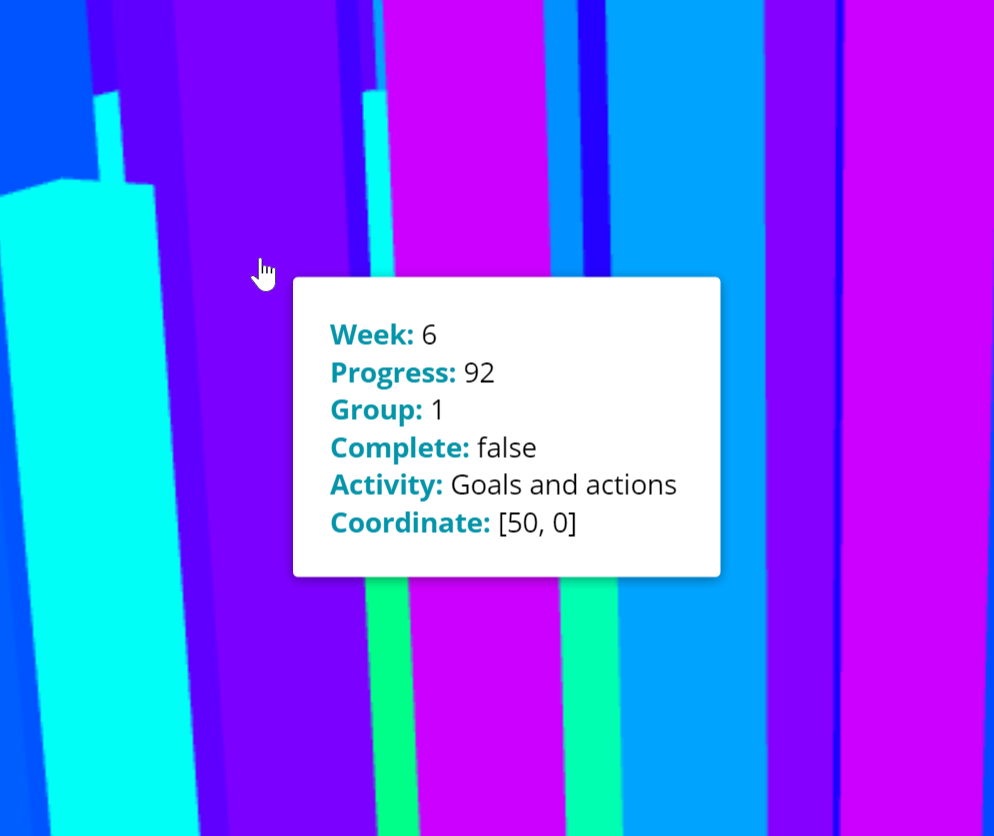
\includegraphics[width=\textwidth]{images/implementation/information_display/student}}
		\caption{Information display for student data.}
		\label{fig:information_display_student}
	\end{subfigure}
	\caption[Information display]{Information display hover effect.}
	\label{fig:information_display}
\end{figure}


}

\todo{Map to project outcomes??}